\chapter{Release front-end}
\label{Chapter3}

Để release các phiên bản khác nhau của front-end, ta chỉ cần tải lên toàn bộ thư mục lên một repository GitHub trống. Cài đặt này mặc định đã tồn tại một tài khoản GitHub và một repository trống.

\section{Tải lên thư mục}
Tại repository trống, tiến hành tải lên toàn bộ thư mục.

\subsection{Tiến hành release}
Tại trang chủ của repository, chọn \texttt{Create a new release} tại mục Release (Xem Hình ~\ref{fig:github_create_release}).
\begin{figure}
    \centering
    
\includegraphics[width=1\linewidth]{github_create_release.png}
    \caption{Mục tạo release mới}
    \label{fig:github_create_release}
\end{figure}

\subsection{Xuất bản Release}
Điền tất cả những thông tin cần thiết cho bản release và chọn Publish Release. (Xem Hình ~\ref{fig:github_publish_release})
\begin{figure}
    \centering
    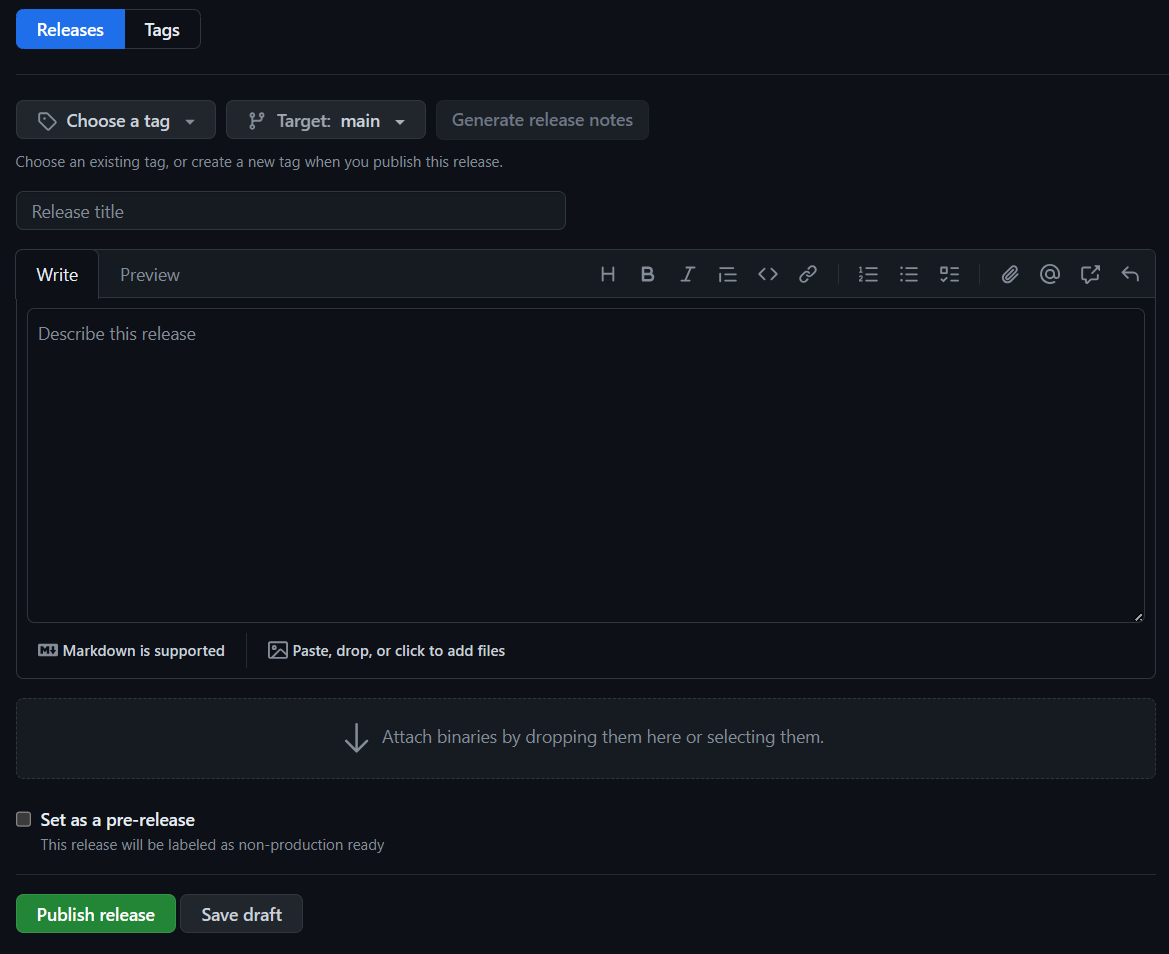
\includegraphics[width=1\linewidth]{github_publish_release.png}
    \caption{Tạo một phiên  bản release}
    \label{fig:github_publish_release}
\end{figure}